\documentclass[12pt]{report} % Times New Roman, 12pt
%\usepackage{gscale_thesis_singlespace} % Single spaced thesis
\usepackage{gscale_thesis_doublespace} % Double spaced thesis
\usepackage{fancyheadings} % Header and footer styling
\usepackage{natbib} % Bibliography formatting
\usepackage{setspace} % Allows double spacing but skips headers/footers
\setcounter{tocdepth}{1} % Limits the TOC to chapter and section names

% Additional packages
\usepackage{graphicx} % Allows the inclusion of figures
\usepackage{subcaption} % Allows captions to be added to subfigures
\usepackage[justification=centering]{caption} % Centres caption text
\usepackage{array} % Used for table formatting
\newcolumntype{P}[1]{>{\raggedright\let\newline\\\arraybackslash\hspace{0pt}}m{#1}}
\usepackage{booktabs} % Fancy-style tables
\usepackage{longtable} % Allows for tables that are more than one page long
\usepackage{float} % Better figure placement control
\usepackage{enumerate} % Numbered lists
\usepackage[shortlabels]{enumitem} % For controlling enumerate labels
\usepackage[shortcuts]{extdash} % Allows manual hyphenation of hypenated words
\usepackage{amsmath} % Non-standard math symbols
\usepackage{amsfonts} % Extended fonts for mathematics

\usepackage[hidelinks]{hyperref} % Linking to LaTeX labels and external URLs

\numberwithin{equation}{section} % Numbers equations based on their section

% ********************************
\begin{document}
\title{Your Thesis Title, Which Can Be As Long As You Want On the Title Page}
\halftitle{Short Title} % 60 Characters Max. Including Spaces

\author{Jane Doe}
\shortauthor{J. Doe} % Used for page header

\dept{Department You Belong To}
\field{Your Field} % What field your thesis is in (e.g. Software Engineering)

\prevdegreeone{B.Eng. (Software Engineering \& Game Design),\\ McMaster University, Hamilton, Canada}
\prevdegreetwo{B.Eng.} % Just your degree's field

\submitdate{MONTH YEAR} % Use the month's full spelling e.g. November
\copyrightyear{YYYY} % Year you are submitting this, usually your graduation 
%year

\doctype{Report} % ``Report'' or ``Thesis'' or whatever you need
\degree{Masters of Engineering} % The degree you get when you submit this
\degreeabbrv{M.Eng.}
\principaladviser{Your Supervisor} % Your Supervisor
 % LaTeX variables for preface pages/headers
    
\beforepreface % Half title page, title page, declaration page   
  \prefacesection{Lay Abstract}

A lay abstract of not more 150 words must be included explaining the key goals and contributions of the thesis in lay terms that is accessible to the general public.  % Lay Abstract
  \prefacesection{Abstract}
Drasil is a framework that generates software, including code, documentation, software requirement specification, user manual, and axillary files. Recently, the Drasil team has been interested in expanding its knowledge to solve higher-order ODEs. In this research, for single higher-order linear ODEs, the Drasil framework can solve them without manually extracted information. For higher-order nonlinear ODEs, the Drasil framework can solve them with manually extracted information.

Firstly, we design a flexible and reusable structure to store ODE information based on conventional mathematical knowledge. This makes it possible to reuse ODE information for documentation and for code generation. Secondly, we provide a commonality analysis of four external ODE solver libraries. The analysis includes how they solve the ODE, what algorithms they use, and what options they provide for different types of output. Thirdly, we enable the Drasil Code Generator to solve nonlinear higher-order ODEs with some manually extracted information. We created a new case study, Double Pendulum, that has a system of higher-order ODE. Further, we solve the Double Pendulum example numerically via external libraries. Lastly, for single higher-order ODEs, the Drasil Code Generator can generate code without manually extracted information.

This research accomplishes three main goals. Firstly, we capture the knowledge of linear ODE in a flexible and reusable structure. Secondly, we expand the Drasil capability to solve higher-order ODEs with/without manually written equations. Solving single higher-order linear ODEs does not require manually extracted information. To solve nonlinear ODEs, manually extracting information from the original ODE is still required. The last one is removing the duplicated information caused by the implementation of solving ODEs. % Abstract
  %\thispagestyle{empty}
\null\vfill
\begin{center}
%\textbf{Dedications}
%\linebreak
\textsl{Your Dedication \\ Optional second line}
\end{center}
\vfill
 % Dedication
  todo
 % Acknowledgements
  \referencepages % Table of Contents, List of Figures, List of Tables
  \prefacesection{Notation, Definitions, and Abbreviations}

\section*{Notation}
\begin{description}[font=\rmfamily\bfseries, leftmargin=3.5cm, style=nextline]
	\item[$\mathbb{R}$] any real number in (-$\infty$, $\infty$).
	\item[$\mathbb{R}^n$] a sequence that contains real numbers, n depends on number of inputs values.
	\item[$\mathbb{R}^i$] a finite sequence that contains real numbers, i depends on the start time, end time, and time step.
	\item[$\mathbb{R}^j$] a infinite sequence that contains real numbers, j is a natural number.
	\item[$\mathbb{R} \rightarrow \mathbb{R}^k$] a function takes an independent variable and outputs a sequence of dependent variables.
\end{description}

\section*{Definitions}
\begin{description}[font=\rmfamily\bfseries, leftmargin=5cm, style=nextline]
	\item[Drasil Framework] references the whole \href{https://jacquescarette.github.io/Drasil/}{Drasil Project}.
	\item[Drasil Code Generator] compile captured knowledge to code.
	\item[Drasil Printer] displays captured knowledge in SRS.
\end{description}

\section*{Abbreviations}
\begin{description}[font=\rmfamily\bfseries, leftmargin=3.5cm, style=nextline]
	\item[ACM] Apache Commons Maths
	\item[BDF] Differentiation Formula Method
	\item[BVP] Boundary Value Problem
	\item[DblPendulum] Double pendulum
	\item[GOOL] Generic Object-Oriented Language
	\item[IVP] Initial Value Problem
	\item[NoPCM] Solar water heating system without PCM
	\item[ODE] Ordinary differential equation
	\item[PDController] Proportional derivative controller
	\item[RK] Runge-Kutta
	\item[SCS] Scientific computing software
	\item[SglPendulum] Single Pendulum
	\item[SRS] Software requirements specification
\end{description}
  \academicstatement{academicachievementdeclaration}
\afterpreface
  
  
  \section{Problem Statement}

In Drasil, we are focused on understanding families of scientific software, and
creating systematic rules to generate families of software solutions (for any
instance of a scientific problem that requires a scientific software solution).
Specifically, Drasil is focused on mathematics and physics-based models. In both
areas, we are concerned with what \textit{kinds of theories} are
well-understood, and ensuring that all created mathematical expressions are
``valid''.

\intodo{Move above paragraph to the top of the ``Drasil'' section.}

\section{Contributions of the Author}

\begin{itemize}
      \item The problem of obtaining more information from our theories so that we
            may make better use from their meta-level information was understood
            before this work.
      \item A partial solution to this problem was also constructed before this
            work.
      \item The expression language used to build theories and, ultimately, inputs
            to outputs was constructed before this work.
\end{itemize}

\section{Thesis Outline}

In \autoref{chap:ideology}, we discuss the focal ideology underpinning this
work, and Drasil. \autoref{chap:drasil} describes Drasil, the host project
carrying the fruits of this work. \autoref{chap:modelkinds} discusses how
theories are encoded in Drasil, the issues associated with using a single
universal mathematical language to describe theories, and how we can resolve
these problems. \autoref{chap:typedExpr} describes residual issues associated
with validating and transcribing mathematical expressions.
\autoref{chap:knowledgeMgmt} continues to discuss the ways in which general
knowledge and theories are encoded in Drasil, and methods for altering their
encoding, leading into \autoref{chap:futureWork}, where we discuss future work.
                  
        \setcounter{figure}{0}
        \setcounter{equation}{0}
        \setcounter{table}{0}
        
  \chapter{Your Chapter Title}

This is a sample chapter

If you need to use quotes, type it ``like this''.

\section{Referencing}
These are some sample references to GAMYGDALA~\citep{popescu2014gamygdala} from 
the \texttt{references.bib} file and state effects of 
cognition~\citep{hudlicka2002time} from the \texttt{references\_another.bib} 
file. These references are not in the same .bib file.

\section{Figures}
This is a single image figure (Figure~\ref{fig_singleenv}):

\begin{figure}[ht]
    \centering
    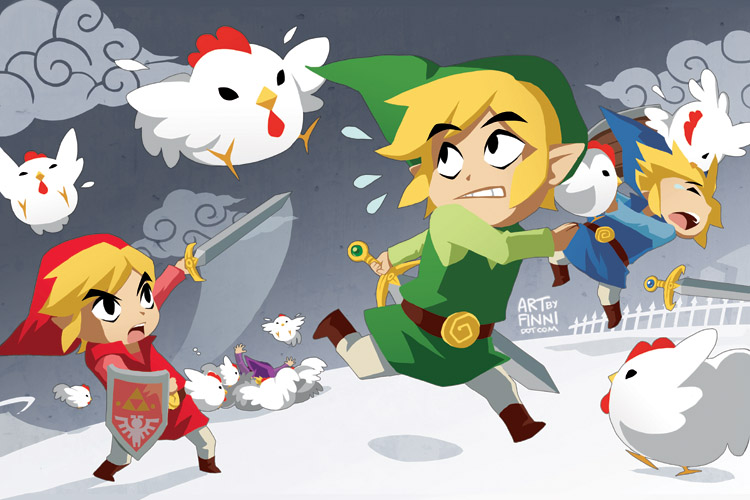
\includegraphics[width=0.6\textwidth]{figures/Sample/tumblr_static_eaceks0rfxsss8o4swscw40wo.jpg}
    \caption[Single Figure Environment Listed Title]{This is a single figure 
    environment}
    \label{fig_singleenv}
\end{figure}

This is a multi-image figure with a top (Figure~\ref{fig_multienv_1}) and bottom (Figure~\ref{fig_multienv_2}) aligned subfigures:

\begin{figure}[ht]
	\centering
	\begin{subfigure}[t]{\textwidth}
		\centering
		
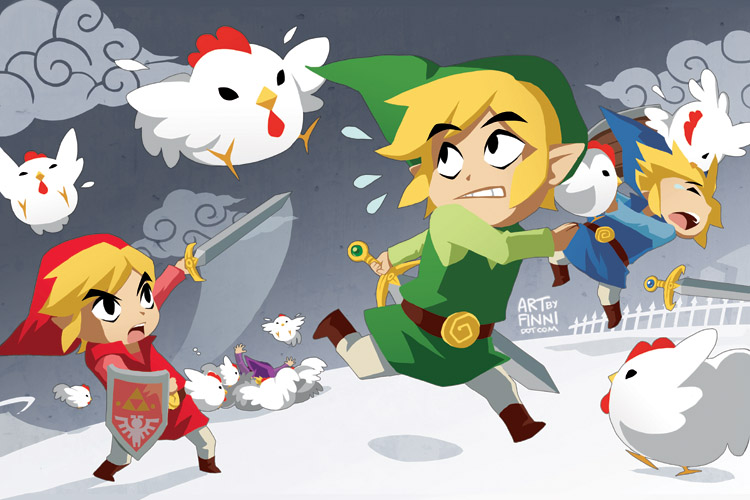
\includegraphics[width=0.7\textwidth]{figures/Sample/tumblr_static_eaceks0rfxsss8o4swscw40wo.jpg}
		\caption{Figure 1}
		\label{fig_multienv_1}
	\end{subfigure}
	~
	\begin{subfigure}[t]{\textwidth}
		\centering
		
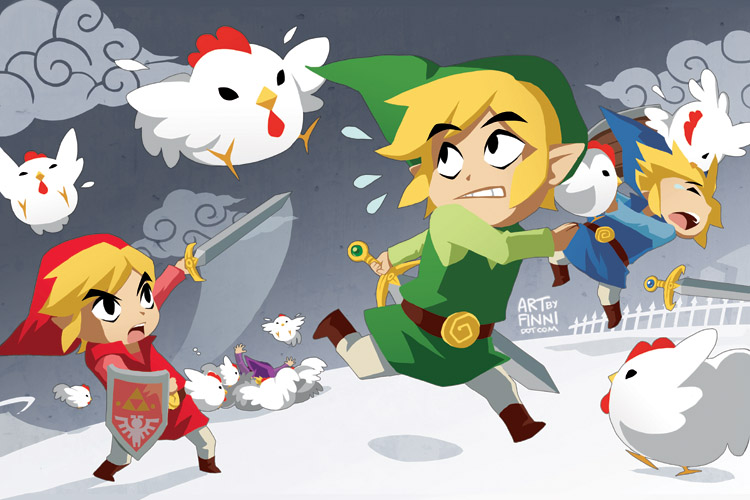
\includegraphics[width=0.7\textwidth]{figures/Sample/tumblr_static_eaceks0rfxsss8o4swscw40wo.jpg}
		\caption{Figure 2}
		\label{fig_multienv_2}
	\end{subfigure}
	
	\caption{A Multi-Figure Environment}
	\label{fig_multienv}
\end{figure}

\section{Tables}

Here is a sample table (Table~\ref{tab_sample}):

	\begin{table}[ht]
	\centering
	\begin{tabular}{ m{0.2\textwidth} m {0.1\textwidth} m{0.15\textwidth} }
		\toprule
		A & $\longleftrightarrow$ & B \\
		C & $\longleftrightarrow$ & D \\
		\bottomrule	
	\end{tabular}	
	\caption{A sample table}	
	\label{tab_sample}
\end{table}

\subsection{Long Tables}
A sample long table is shown in Appendix~\ref{appendix_b}.

\section{Equations}

Here is a sample equation (Equation~\ref{eq_lineslope}):

\begin{equation} \label{eq_lineslope}
	y = mx + b
\end{equation}                  
       \setcounter{figure}{0}
       \setcounter{equation}{0}
       \setcounter{table}{0}

  \chapter{Conclusion}
An ODE is a type, and it exists in many forms. Previously to this research, the Drasil Framework had no flexible and reusable structure for capturing ODE information. The Drasil teams have to manually extract useful information from the original ODE to instruct the Drasil Code Generator to generate code. This approach propagates duplicated information and loses traceability. The newly created structure, \verb|DifferentialModel|, stores linear ODE information based on the conventional matrix concept. It provides the flexibility to transform a linear ODE from one form to another mathematically equivalent form. Once we capture the knowledge of ODE in the new structure, we can reuse it for other purposes, such as producing the numerical solution and displaying the ODE.

Along with \verb|DifferentialModel|, four selected external libraries are responsible for producing the numerical solution for a system of first-order ODEs. Drasil users can get a numerical solution by choosing an algorithm. Currently, although the Calculations module outputs a finite stream of real numbers, $\mathbb{R}^m$, there are other design options. The C\# OSLO provides an option to output an infinite stream of real numbers, $\mathbb{R}^{\infty}$. It has richer data than $\mathbb{R}^m$. Also, outputting the ODE as a function that can return the value of the dependent variable for any value of the independent variable could help generate libraries in Drasil. We did not complete implementing the new specifications for this, but the analysis provides a starting point for future research.

\verb|DifferentialModel| provides reusable ODE information, and external libraries provide mathematical knowledge for solving the ODE. Before we bridge the gap between \verb|DifferentialModel| and external libraries, we enable solving any higher-order ODEs with manually written equations via external libraries. The Double Pendulum case study demonstrates the Drasil Framework can generate code that solves a system of higher-order non-linear ODEs. With all implementations, we are ready to bridge the gap by automating the process of extracting useful information from \verb|DifferentialModel| and then forming an \verb|ODEInfo|. While we are solving a single higher-order linear ODE, we generate it instead of manually writing \verb|ODEInfo|. The automation removes the duplicated information and potentially increases traceability.

This research accomplishes three main goals. Firstly, we capture the knowledge of ODE in a flexible and reusable structure. Secondly, we expand the Drasil capability to solve any higher-order ODEs with manually written equations. The last one is removing the duplicated information caused by the implementation of solving ODEs.

        \setcounter{figure}{0}
        \setcounter{equation}{0}
        \setcounter{table}{0}

\begin{appendix}
    \chapter{Your Appendix}
\label{appendix_a}

This appendix provides detailed explanations of various parts of DifferentialModel.

\section{Constructors of DifferentialModel}
\label{const_de}

% \begin{listing}[ht]
\begin{haskell1}
-- $K_d$ is qdDerivGain
-- $y_t$ is opProcessVariable
-- $K_p$ is qdPropGain
-- $r_t$ is qdSetPointTD
imPDRC :: DifferentialModel
imPDRC = makeASingleDE
	time
	opProcessVariable
	lhs
	rhs
	"imPDRC"
	(nounPhraseSP "Computation of the Process Variable as a function of time")
	EmptyS
	where 
	lhs = [exactDbl 1 `addRe` sy qdDerivGain $* (opProcessVariable $^^ 1)]
	$+ (exactDbl 1 $* (opProcessVariable $^^ 2))
	$+ (exactDbl 20 `addRe` sy qdPropGain $* (opProcessVariable $^^ 0))
	rhs = sy qdSetPointTD `mulRe` sy qdPropGain
\end{haskell1}
\captionof{listing}{Using input language for the example~\ref{eq_odeexmaple} in DifferentialModel}
% \label{code_scexinputl}
% \end{listing}

% \begin{listing}[ht]
\begin{haskell1}
imPDRC :: DifferentialModel
imPDRC = makeASystemDE
	time
	opProcessVariable
	coeffs = [[exactDbl 1, exactDbl 1 `addRe` sy qdDerivGain, exactDbl 20 `addRe` sy qdPropGain]]
	unknowns = [2, 1, 0]
	constants = [sy qdSetPointTD `mulRe` sy qdPropGain]
	"imPDRC"
	(nounPhraseSP "Computation of the Process Variable as a function of time")
	EmptyS
\end{haskell1}
\captionof{listing}{Explicitly set values for the example~\ref{eq_odeexmaple} in DifferentialModel}
% \label{code_scexmatrix}
% \end{listing}

\section{Numerical Solution Implementation}
\label{numsol}

% \begin{listing}[ht]
\begin{python1}
def func_y_t(K_d, K_p, r_t, t_sim, t_step):
    def f(t, y_t):
        return [y_t[1], -(1.0 + K_d) * y_t[1] + -(20.0 + K_p) * y_t[0] + r_t * K_p]
    
    r = scipy.integrate.ode(f)
    r.set_integrator("dopri5", atol=Constants.Constants.AbsTol, rtol=Constants.Constants.RelTol)
    r.set_initial_value([0.0, 0.0], 0.0)
    y_t = [[0.0, 0.0][0]]
    while r.successful() and r.t < t_sim:
        r.integrate(r.t + t_step)
        y_t.append(r.y[0])
    
    return y_t
\end{python1}
\captionof{listing}{Source code of solving PDController in Scipy}
% \label{code_pythonscipy}
% \end{listing}

In line 1, \verb|func_y_t| is a function output the numerical solution, and it is a list of numbers. In the line 2, the local function \verb|f| contains ODE. The line 3 shows local function return a list. Since we want to solve a system of ODE, the index one is the first ODE in this system, and the index two is the second ODE this system. By calling \verb|scipy.integrate.ode|, we pack ODE information in the generic interface. The line between 5 and 10, are procedure how to set configuration and collecting results. Theoretically, we can just return the \verb|r| in line 4 to present returning a function of ODE.

% \begin{listing}[ht]
\begin{java1}
public static ArrayList<Double> func_y_t(double K_d, double K_p, double r_t, double t_sim, double t_step) {
	ArrayList<Double> y_t;
	ODEStepHandler stepHandler = new ODEStepHandler();
	ODE ode = new ODE(K_p, K_d, r_t);
	double[] curr_vals = {0.0, 0.0};

	FirstOrderIntegrator it = new DormandPrince54Integrator(t_step, t_step, Constants.AbsTol, Constants.RelTol);
	it.addStepHandler(stepHandler);
	it.integrate(ode, 0.0, curr_vals, t_sim, curr_vals);
	y_t = stepHandler.y_t;

	return y_t;
}
\end{java1}
\captionof{listing}{A linear system of first-order representation in ACM}
% \label{code_javaacm}
% \end{listing}

% \begin{listing}
\begin{cplusplus1}
vector<double> func_y_t(double K_d, double K_p, double r_t, double t_sim, double t_step) {
	vector<double> y_t;
	ODE ode = ODE(K_p, K_d, r_t);
	vector<double> currVals{0.0, 0.0};
	Populate pop = Populate(y_t);
		
	boost::numeric::odeint::runge_kutta_dopri5<vector<double>> rk = boost::numeric::odeint::runge_kutta_dopri5<vector<double>>();
	auto stepper = boost::numeric::odeint::make_controlled(Constants::AbsTol, Constants::RelTol, rk);
	boost::numeric::odeint::integrate_const(stepper, ode, currVals, 0.0, t_sim, t_step, pop);
	
	return y_t;
}	
\end{cplusplus1}
\captionof{listing}{A linear system of first-order representation in ODEINT}
% \label{code_cplusplusodeint}
% \end{listing}

% \begin{listing}[ht]
\begin{csharp1}
public static List<double> func_y_t(double K_d, double K_p, double r_t, double t_sim, double t_step) {
	List<double> y_t;
	Func<double, Vector, Vector> f = (t, y_t_vec) => {
		return new Vector(y_t_vec[1], -(1.0 + K_d) * y_t_vec[1] + -(20.0 + K_p) * y_t_vec[0] + r_t * K_p);
	};
	Options opts = new Options();
	opts.AbsoluteTolerance = Constants.AbsTol;
	opts.RelativeTolerance = Constants.RelTol;
	
	Vector initv = new Vector(new double[] {0.0, 0.0});
	IEnumerable<SolPoint> sol = Ode.RK547M(0.0, initv, f, opts);
	IEnumerable<SolPoint> points = sol.SolveFromToStep(0.0, t_sim, t_step);
	y_t = new List<double> {};
	foreach (SolPoint sp in points) {
		y_t.Add(sp.X[0]);
	}
	
	return y_t;
}
\end{csharp1}
\captionof{listing}{Source code of solving PDController in OSLO}
% \label{code_csharposlo}
% \end{listing}


\section{Algorithm in External Libraries}
\label{alg_externallib}

\begin{table}[ht]
\begin{tabular}{ p{0.2\textwidth} p{0.7\textwidth} }
	\textbf{Name} & \textbf{Description} \\
	\toprule
	\verb|zvode| & Complex-valued Variable-coefficient Ordinary Differential Equation solver, with fixed-leading-coefficient implementation. It provides implicit Adams method (for non-stiff problems) and a method based on backward differentiation formulas (BDF) (for stiff problems).\\ \hline
	\verb|lsoda| & Real-valued Variable-coefficient Ordinary Differential Equation solver, with fixed-leading-coefficient implementation. It provides automatic method switching between implicit Adams method (for non-stiff problems) and a method based on backward differentiation formulas (BDF) (for stiff problems).\\ \hline
	\verb|dopri5| & This is an explicit runge-kutta method of order (4)5 due to Dormand \& Prince (with stepsize control and dense output).\\ \hline
	\verb|dop853| & This is an explicit runge-kutta method of order 8(5,3) due to Dormand \& Prince (with stepsize control and dense output).\\
	\bottomrule	
\end{tabular}	
\caption{Algorithm Options in Scipy~\citep{scipyfun}}	
\label{tab_algscipy}
\end{table}

\begin{table}[ht]
\begin{tabular}{ p{0.27\textwidth} p{0.7\textwidth} }
	\textbf{Name} & \textbf{Description} \\
	\toprule
	\verb|Euler| & This class implements a simple Euler integrator for Ordinary Differential Equations.\\ \hline
	\verb|Midpoint| & This class implements a second order Runge-Kutta integrator for Ordinary Differential Equations.\\ \hline
	\verb|Classical RungeKutta| & This class implements the classical fourth order Runge-Kutta integrator for Ordinary Differential Equations (it is the most often used Runge-Kutta method).\\ \hline
	\verb|Gill| & This class implements the Gill fourth order Runge-Kutta integrator for Ordinary Differential Equations.\\ \hline
	\verb|Luther| & This class implements the Luther sixth order Runge-Kutta integrator for Ordinary Differential Equations.\\ \hline
	\verb|Higham and Hall| & This class implements the 5(4) Higham and Hall integrator for Ordinary Differential Equations.\\ \hline
	\verb|DormandPrince 5(4)| & This class implements the 5(4) Dormand-Prince integrator for Ordinary Differential Equations.\\ \hline
	\verb|DormandPrince 8(5,3)| & This class implements the 8(5,3) Dormand-Prince integrator for Ordinary Differential Equations.\\ \hline
	\verb|Gragg-Bulirsch-Stoer| & This class implements a Gragg-Bulirsch-Stoer integrator for Ordinary Differential Equations.\\ \hline
	\verb|Adams-Bashforth| & This class implements explicit Adams-Bashforth integrators for Ordinary Differential Equations.\\ \hline
	\verb|Adams-Moulton| & This class implements implicit Adams-Moulton integrators for Ordinary Differential Equations.\\
	\bottomrule	
\end{tabular}	
\caption{Algorithm Options in Apache Commons Maths~\citep{apachefun}}	
\label{tab_algacm}
\end{table}

\begin{table}[ht]
\begin{tabular}{ p{0.4\textwidth} p{0.5\textwidth} }
	\textbf{Name} & \textbf{Description} \\
	\toprule
	\verb|euler| & Explicit Euler: Very simple, only for demonstrating purpose\\ \hline
	\verb|runge_kutta4| & Runge-Kutta 4: The classical Runge Kutta scheme, good general scheme without error control.\\ \hline
	\verb|runge_kutta_cash_karp54| & Cash-Karp: Good general scheme with error estimation.\\ \hline
	\verb|runge_kutta_dopri5| & Dormand-Prince 5: Standard method with error control and dense output.\\ \hline
	\verb|runge_kutta_fehlberg78| & Fehlberg 78: Good high order method with error estimation.\\ \hline

	\verb|adams_bashforth_moulton| & Adams-Bashforth-Moulton: Multi-step method with high performance.\\ \hline
	\verb|controlled_runge_kutta| & Controlled Error Stepper: Error control for the Runge-Kutta steppers.\\ \hline
	\verb|dense_output_runge_kutta| & Dense Output Stepper: Dense output for the Runge-Kutta steppers.\\ \hline
	\verb|bulirsch_stoer| & Bulirsch-Stoer: Stepper with step size, order control and dense output. Very good if high precision is required..\\ \hline
	\verb|implicit_euler| & Implicit Euler: Basic implicit routine.\\ \hline
	\verb|rosenbrock4| & Rosenbrock 4: Solver for stiff systems with error control and dense output.\\ \hline
	\verb|symplectic_euler| & Symplectic Euler: Basic symplectic solver for separable Hamiltonian system.\\ \hline
	\verb|symplectic_rkn_sb3a_mclachlan| & Symplectic RKN McLachlan: Symplectic solver for separable Hamiltonian system with order 6.\\
	\bottomrule	
\end{tabular}	
\caption{Algorithm Options in ODEINT~\citep{odeintfun}}	
\label{tab_algodeint}
\end{table}

\begin{table}[ht]
\begin{tabular}{ p{0.2\textwidth} p{0.7\textwidth} }
	\textbf{Name} & \textbf{Description} \\
	\toprule
	\verb|RK547M| & This method is most appropriate for solving non-stiff ODE systems. It is based on classical Runge-Kutta formulae with modifications for automatic error and step size control.\\ \hline
	\verb|GearBDF| & It is an implementation of the Gear back differentiation method, a multi-step implicit method for stiff ODE systems solving.\\
	\bottomrule	
\end{tabular}	
\caption{Algorithm Options in OSLO~\citep{oslofun}}	
\label{tab_algodeint}
\end{table}

        \setcounter{figure}{0}
        \setcounter{equation}{0}
        \setcounter{table}{0}

    \chapter{Long Tables}
\label{appendix_b}

This appendix demonstrates the use of a long table that spans multiple pages.

\begin{center}
\begin{longtable}{P{3cm}P{3cm}P{2.5cm}P{3.5cm}}
\toprule
\hline
\textbf{Col A} & \textbf{Col B} & \textbf{Col C} & \textbf{Col D} \\ \midrule

\endfirsthead
\multicolumn{4}{c}{\textit{Continued from previous page}} \\ \hline
\textbf{Col A} & \textbf{Col B} & \textbf{Col C} & \textbf{Col D} \\ \hline
\endhead
\hline \multicolumn{4}{r}{\textit{Continued on the next page}} \\
\endfoot
\hline
\endlastfoot

A & B & C & D \\ \midrule

A & B & C & D \\ \midrule

A & B & C & D \\ \midrule

A & B & C & D \\ \midrule

A & B & C & D \\ \midrule

A & B & C & D \\ \midrule

A & B & C & D \\ \midrule

A & B & C & D \\ \midrule

A & B & C & D \\ \midrule

A & B & C & D \\ \midrule

A & B & C & D \\ \midrule

A & B & C & D \\ \midrule

A & B & C & D \\ \midrule

A & B & C & D \\ \midrule

A & B & C & D \\ \midrule

A & B & C & D \\ \midrule

A & B & C & D \\ \midrule

A & B & C & D \\ \midrule

A & B & C & D \\ \midrule

A & B & C & D \\ \midrule

\hline
\end{longtable}
\end{center}

        \setcounter{figure}{0}
        \setcounter{equation}{0}
        \setcounter{table}{0}
\end{appendix}

% The bibliography is set up to allow for multiple bib files
\bibliographystyle{ACM-Reference-Format}
\bibliography{references,references_another}

\label{NumDocumentPages}

\end{document}
% ********************************
